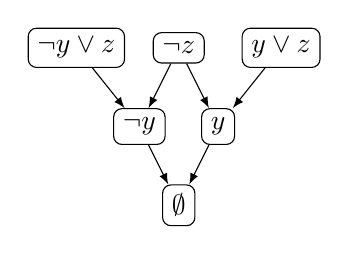
\begin{tikzpicture}[>=latex]
    \node[rectangle, rounded corners = 3pt, draw] (a) at (-1.3, 2)
        {$\neg y \lor z$};
    \node[rectangle, rounded corners = 3pt, draw] (a2) at (1.3, 2)
        {$y \lor z$};
    \node[rectangle, rounded corners = 3pt, draw] (b) at (0, 2)
        {$\neg z$};
    \node[rectangle, rounded corners = 3pt, draw] (c) at (-0.5, 1)
        {$\neg y$};
    \node[rectangle, rounded corners = 3pt, draw] (d) at (0.5, 1)
       {$y$};
    \node[rectangle, rounded corners = 3pt, draw] (e) at (0, 0)
        {$\emptyset$};

    \draw[->] (a) -- (c);
    \draw[->] (a2) -- (d);
    \draw[->] (b) -- (c);
    \draw[->] (b) -- (d);
    \draw[->] (c) -- (e);
    \draw[->] (d) -- (e);
\end{tikzpicture}